%!TEX root = nips2015.tex
\section{Evaluation of Network Parameters}

\subsection*{Parameter Tuning and Results}

Once the DQN trainer was interfaced with GnuGo, we began adjusting the parameters to more closely mirror those of Clark \& Storkey's DCNN. In this section we discuss the network parameters we tried and the results we were able to achieve with them. To test any given set of parameters, we trained the network for ~30 games and observed the opponent's score. We focused on the opponent's score because we expected that, as the network improved its tactics, the changes would manifest in the GnuGo opponent having more difficulty scoring higher points.

We first reduced Sprague's default training parameters by 4x to account for the fact that, in the Atari case, the network would receive 4 frames at once from ALE, whereas with GnuGo it was receiving one board state at a time. Table \ref{} gives the various parameters we attempted to tune and the specific settings we tried.

We also attempted to integrate weight tying, which was used in the prior DCNN to force the network to take advantage of board symmetry by tying weights together within the convolutional layers. However, doing this with the tools provided by Theano / Lasagne proved very challenging. In the end, we were not able to find a straightforward way to implement this feature in the time allotted. This was a disappointment because intuitively this kind of understanding would help the agent greatly (and this intuition was borne out in Clark \& Storkey's work, which found that incorporating symmetry did increase performance.)

Another issue that proved to be surprisingly challenging, as previously mentioned, was to find a way to prevent the agent from making illegal moves. \textcolor{red}{AM: didn't have time to add the board errors discussion and graph yet.}

Unfortunately, in all cases we were unable to get consistent performance, regardless of specific parameter settings. Figure \ref{fig:score} shows one particular training session that we allowed to run for several hundred epochs. 

\begin{figure}[h!]
\centering
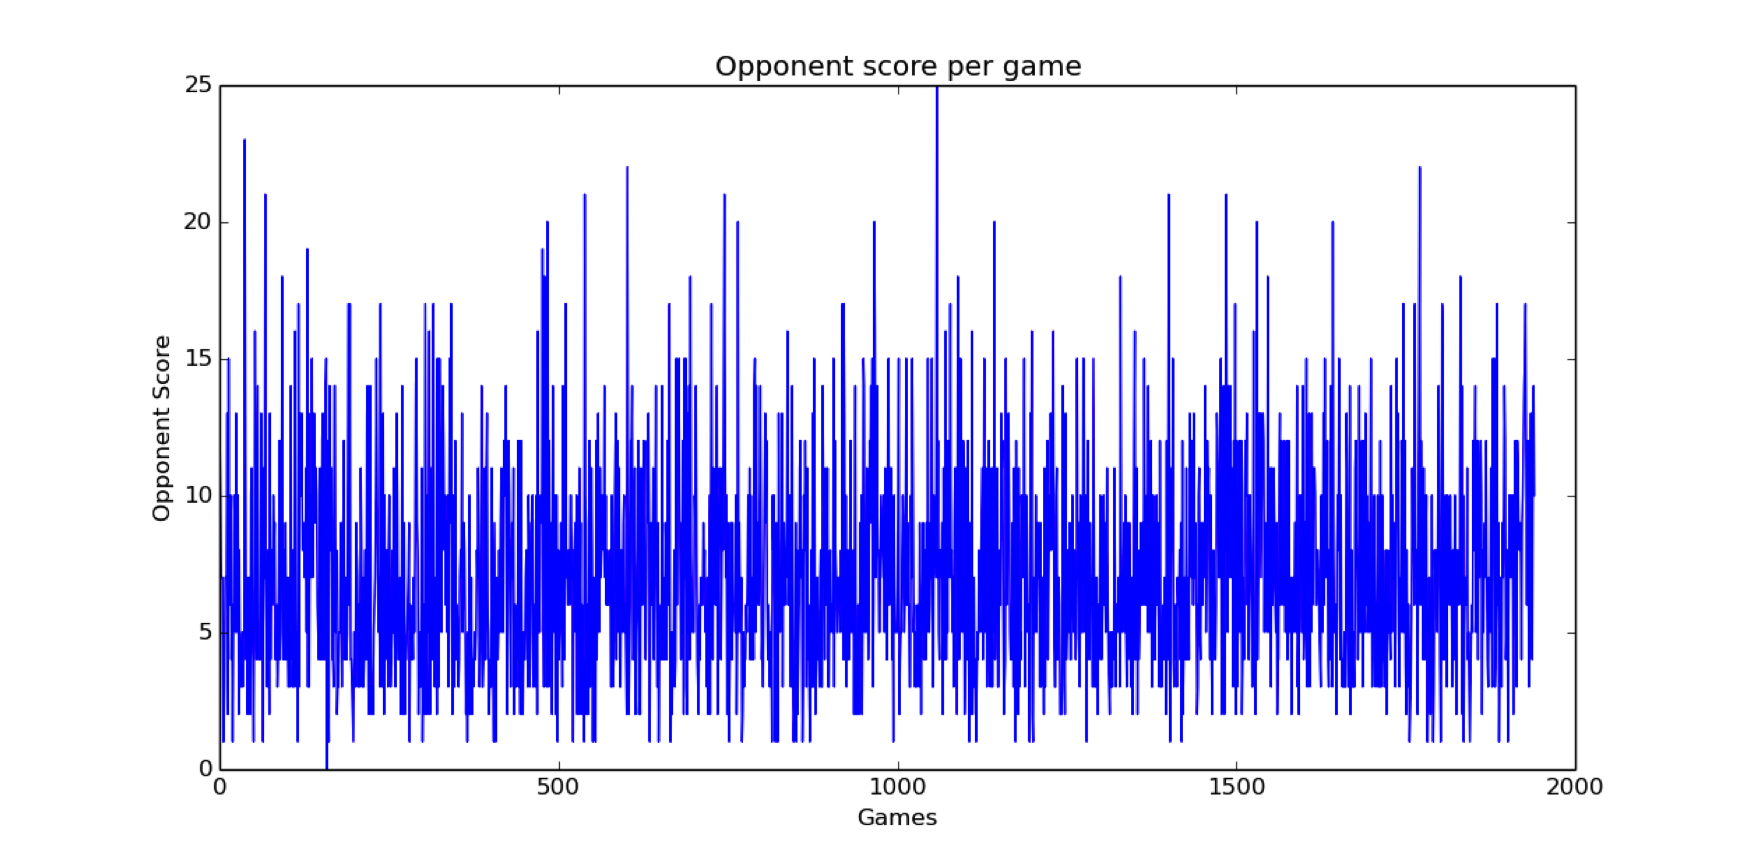
\includegraphics[scale=0.5]{training_score.png}
\caption{Opponent (GnuGo) score per training epoch.}
\label{fig:score}
\end{figure}


\textcolor{red}{AM: need some analysis on why it didn't work... could possibly migrate this into the Future Work section instead.}